\chapter{Gestion du projet}
\section{Organisation du projet}
Dès le départ, nous avons décidé de travailler avec git, plus précisement 
en utilisant le site \url{https://github.com}. Nous avons donc créé une organisation afin de séparer les différents dépots. Nous en avons définis 2, mais les membres de l'organisation étaient libres d'en ajouter d'autres.
\begin{itemize}
    \item crapauduc. Ce dépôt est le dépot principal où les notebooks des modèles sont déposés, nous y avons aussi placé les rapports des anciens étudiants afin d'y avoir un accès rapide. Nous y avons aussi déposé un subset d'image d'environ 0.5 Gib permettant le fine tuning.
    \item utils. Ce dépôt contient des scripts faisant des transformations ou des analyses sur les données. Nous y avons par exemple un script qui permet de convertir les annotations de csv à COCO.
\end{itemize}

De plus, nous avons créé un compte google ayant le doux nom de \verb|student GML| afin d'avoir un espace google drive de 15 GiB pour se partager aisément les données ainsi qu'une intégration facilitée dans le service \url{colab.research.google.com} de Google. Cependant, cette organisation n'a pas été complètement satisfaisante comme détaillé dans les points suivants.


\section{Gestion du temps de travail}
Dès le départ, nous avons décidé de travailler à distance afin de dédier 
la totalité de la journée à ce projet sans perdre de temps dans les transports publiques. En effet, le mardi où tombe le cours de GML, nous n'avons pas d'autre cours que ce dernier. Ainsi, un mardi typique se déroule comme suit:
\begin{itemize}
    \item 8h00 - 13h15: Libre, mais souvent on prépare la séance de l'après-midi.
    \item 13h15 - 15h: Appel Teams, où nous expliquons notre avancement, normalement les différents problèmes rencontrés durant la semaine doivent être réglé avant la réunion. Planification des tâches pour la prochaine semaine, et répartition des tâches. Durant chaque réunion un membre du groupe prend des notes afin d'avoir un historique des discussions, ce procès verbale des réunions est stocké sur le google drive de \verb|student GML|.
    \label{item:seance}
\end{itemize}
La séance du mardi se résume donc essentiellement à un partage d'informations entre les différents groupes de travail composés de 1 à 3 étudiant.e.s. Le travail proprement dit est pour la plupart effectué en dehors des réunions, soit le mardi après la réunion soit à un autre moment choisit par les membres du groupe.

\section{Gestion des tâches et répartition}
Nous avons poussé notre utilisation de github, en gérant nos tâches à l'aide de l'outil de gestion de projet \href{https://github.com/topics/kanban}{kanban} directement intégré dans github. Ainsi, nous pouvons savoir à n'importe quel moment quel membre de l'équipe travail sur quelle partie du projet. De plus, nous pouvons voir les tâches en cours, les tâches terminées, les tâches en attentes, etc. 

\begin{figure}[htb!]
    \centering
    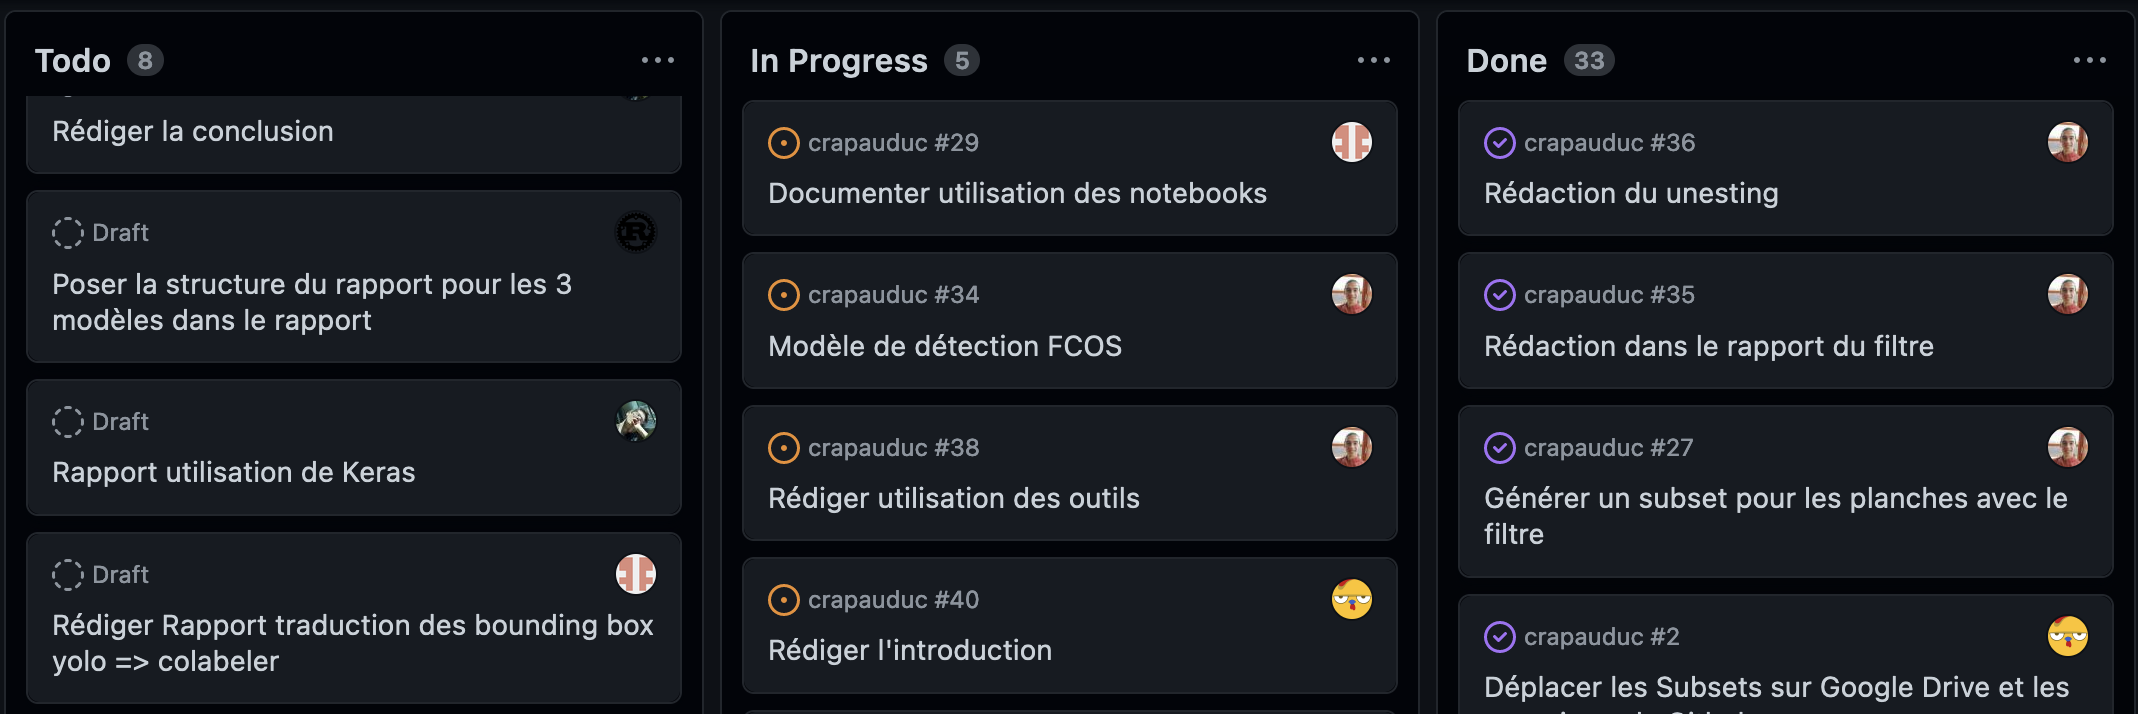
\includegraphics[width=0.8\linewidth]{images/kanban.png}
    \caption{Nos tâches du Kanban réparties en 3 catégories : à faire, en cours et terminées.}
    \label{fig:kanban}
\end{figure}

\paragraph{Problèmes d'organisation:} Nous avons décidé de ne pas élire de responsable au sein des étudiants et de garder une hiérarchie horizontale. Cette décision a bien fonctionné pour certains aspects du travail, comme par exemple: la prise des notes durant les réunions.
Cependant les appels Teams étaient généralement coordonnés par Olivier et Joris sans vraiment que cela ait été expressément prévu. Cette manière de fonctionner s'est imposé naturellement et nous avons gardé cette organisation pour la suite. Par coordination nous entendons de manière générale animer la discussion et amorcer les points suivants. 
L'organisation de travail à elle aussi subit des changements au cours du projet. Au début, nous avons travaillé de manière très individuelle sur les petites tâches initiales. Nous souhaitions pouvoir travailler de manière très parallèle et ce choix semblait être bon.
Néanmoins, cette approche s'est avérée contenir plusieurs problèmes:
\begin{enumerate}
    \item Échanges inefficaces \label{item:friction}
    \item Tâches trop complexes pour une seule personne. \label{item:complex}
\end{enumerate}
Notre organisation initiale fonctionnait bien au début du projet puisque nous avions beaucoup de petites tâches et nous avons bien avancé. 
Cependant, les tâches devenants de plus en plus grosses, les réunions ont pris de plus en plus de temps. 
En effet, nous avons rencontré beaucoup de problèmes qui étaient difficiles à résoudre seul, nous en discutions donc durant les réunions, et celles-ci commençait à prendre trop de temps.
Après quelques séances peu efficaces, nous avons réalisé qu'il serait plus judicieux de séparer le travail en petits groupes afin qu'une partie de la communication se fasse déjà entre les membres du sous-groupe et ainsi que l'on réduise les informations à partager lors des réunions. De plus travailler à plusieurs permettait de surmonter les problèmes rencontrés plus facilement.
\paragraph{}

Un point que nous remarquons après ce travail et le suivant : nous avons souvent débloqué des problèmes en les abandonnant puis en y revenant plus tard, ceci nous a permis d'aborder le problème une seconde fois avec de nouvelles connaissances qui nous ont fait avoir une deuxième approche différente de la première.
\\
Avec notre organisation actuelle, c'est à dire une réunion par semaine, nous n'arrivions pas forcément bien à laisser quelques jours le problème pour y revenir à tête reposée. Nous pensons que faire des réunions moins régulièrement, toutes les deux semaines par exemple, permettrait d'avoir plus de temps et ainsi de retravailler plusieurs fois le même problème entre deux réunions. Cependant cette solution demande des membres du groupe une plus grande autonomie, néanmoins en alliant cette proposition avec les petits groupes de travail présentés précédemment nous pensons que ça peut donner de bons résultats.

\paragraph{}
Un autre problème qui nous a entravé le bon déroulement du projet et spécialement la fin est le manque de ressources. Nous avons commencé par travailler en local, sur nos propres machines. Cependant, nous sommes très vite passés à Atlas afin de pouvoir héberger l'entièreté des données (500GiB) proche des notebooks. Atlas est une machine fournie par les professeurs sur laquelle un serveur Jupyter tournait. Cependant, nous n'avions pas accès à git depuis cet ordinateur ce qui posait des problèmes pour garder le projet synchronisé entre nos ordinateurs, github et Atlas. De plus, une fois les différentes analyses préliminaires terminées, il n'était absolument pas suffisant pour faire un entrainement d'un modèle comme DETR (60+ millions de paramètres). Nous avons donc migré sur l'offre gratuite de Google Colab. Les entrainements nécessitants toujours plusieurs dizaines de minutes, nous avons décidé de payer Colab Pro afin d'avoir accès a des GPUs premiums 
et de pouvoir tester et fine tuner rapidement des modèles. Nous avons donc entrainé plusieurs modèles sur Colab Pro, et les avons évalués avec le benchmark COCO, ceci est expliqué plus en détail dans le chapitre \ref{chap:Evaluation}. Le soucis est le suivant, en ayant déplacé le projet sur plusieurs infrastructures, nous avons eu un projet éparpillé où il était dur de retrouver la dernière version. Un autre point notable est le manque de crédit à la fin du projet ce qui nous a empêché de réaliser certaines analyses. En effet, DETR est tellement gros qu'il ne peut pas être chargé en mémoire sur un GPU non premium. Ainsi certaines expériences que nous aurions pu réaliser n'ont pas été concretisées par manque de moyens. Nous voulions par exemple réaliser une centaine de prédictions sur un nouveau set et faire une fonction qui permet de filtrer certaines prédictions.
\paragraph{} En conclusion, nous sommes satisfait de l'organisation et du déroulement de ce projet, tous les membres du groupe ont travaillé sur des parties diverses et variées du projet. Tout le monde a ainsi pu expérimenter avec au moins un modèle de machine learning. De plus, la gestion s'est faite de manière naturelle et a permit de garder une bonne entente entre les différents étudiants même durant les moments où nous rencontrions des problèmes. Nous sommes particulièrement fiers d'avoir su adapter notre organisation au cours du projet, afin de le mener à bien et ce malgré notre manque de connaissance évident dans le domaine.